%%% Template originaly created by Karol Kozioł (mail@karol-koziol.net) and modified for ShareLaTeX use

\documentclass[a4paper,11pt]{article}

\usepackage[T1]{fontenc}
\usepackage[utf8]{inputenc}
\usepackage{graphicx}
\usepackage{xcolor}
\usepackage[export]{adjustbox}
\usepackage{titlesec}
\usepackage{sectsty}
\allsectionsfont{\sffamily}

\usepackage{tgheros}
\usepackage[defaultmono]{droidmono}
\usepackage{mathptmx}

\usepackage{amsmath,amssymb,amsthm,textcomp}
\usepackage{enumerate}
\usepackage{multicol}
\usepackage{tikz}
\usepackage{tabto}
\usepackage{pxfonts}
\usepackage{geometry}
\geometry{left=25mm,right=25mm,%
bindingoffset=0mm, top=20mm,bottom=20mm}


\linespread{1.2}
\makeatletter
\renewcommand\tableofcontents{%
    \section*{\makebox[\linewidth][c]{\contentsname}%
      \@mkboth{\MakeUppercase\contentsname}{\MakeUppercase\contentsname}}%
    \begin{multicols}{2}%
    \@starttoc{toc}%
    \end{multicols}
    }
\makeatother
\newcommand{\linia}{\rule{\linewidth}{0.5pt}}

% custom theorems if needed
\newtheoremstyle{mytheor}
    {1ex}{1ex}{\normalfont}{0pt}{\scshape}{.}{1ex}
    {{\thmname{#1 }}{\thmnumber{#2}}{\thmnote{ (#3)}}}

\theoremstyle{mytheor}
\newtheorem{defi}{Definition}
\newtheoremstyle{mytheor}
    {1ex}{1ex}{\normalfont}{0pt}{\scshape}{|}{1ex}
    {{\thmname{#1 }}{}{\thmnote{ (#3)}}}

\theoremstyle{mytheor}
\newtheorem{nb}{Please Note}
% my own titles
\makeatletter
\renewcommand{\maketitle}{
\begin{center}
\vspace{2ex}
{\huge \textsf{\textbf{\@title}}}
\vspace{1ex}
\\
\linia\\
\textsf{\@date \hfill
\@author}
\vspace{4ex}
\end{center}
}
\makeatother
%%%

% custom footers and headers
\usepackage{fancyhdr}
\pagestyle{fancy}
\lhead{}
\chead{}
\rhead{}
\lfoot{Assignment 3}
\cfoot{}
\rfoot{Page \thepage}
\renewcommand{\headrulewidth}{0pt}
\renewcommand{\footrulewidth}{0pt}
%

% code listing settings
\usepackage{listings}
\usepackage[space=true]{accsupp}

\definecolor{codegreen}{rgb}{0,0.6,0}
\definecolor{codegray}{rgb}{0.5,0.5,0.5}
\definecolor{inlinecode}{rgb}{0.1,0.1,0.1}
\definecolor{codepurple}{rgb}{0.58,0,0.82}
\definecolor{backcolour}{rgb}{0.95,0.95,0.92}
\lstset{
    language=C,
    basicstyle=\ttfamily\small,
    aboveskip={1.0\baselineskip},
    breakatwhitespace=false,         
    keepspaces=true,
    belowskip={1.0\baselineskip},
    columns=fullflexible,
    extendedchars=true,
    breaklines=true,
    tabsize=4,
    frame=lines,
    showtabs=false,
    showspaces=false,
    showstringspaces=false,
    commentstyle=\color{codegray},
    keywordstyle=\bfseries,
    stringstyle=\rmfamily,
    numbers=left,
    numberstyle=\color{codegray}\footnotesize\noncopynumber,
    stepnumber=1,
    numbersep=10pt,
    captionpos=t,
    escapeinside={\%*}{*)},
}

\newcommand{\noncopynumber}[1]{
    \BeginAccSupp{method=escape,ActualText={}}
    #1
    \EndAccSupp{}
}
\lstdefinestyle{output}{
    basicstyle=\ttfamily\small,
    aboveskip={1.0\baselineskip},
    breakatwhitespace=false,         
    keepspaces=true,
    belowskip={1.0\baselineskip},
    columns=fullflexible,
    extendedchars=true,
    breaklines=true,
    tabsize=4,
    frame=lines,
    showtabs=false,
    showspaces=false,
    showstringspaces=false,
    captionpos=t
}
%%%----------%%%----------%%%----------%%%----------%%%

\begin{document}

\title{CSE-016 Programming Lab Assignment \textnumero{} 3}

\date{15/04/2024}

\author{Youssef Ahmed Samy Kassem\\ \hfill ID 9545 -- Group 3 -- Lab 1\\ \hfill SSP -- Faculty of Engineering, Alexandria University\\}

\maketitle
\textsf{\textsl{\textbf{Solutions begin from the second page.}}}
\section{Problems}
\subsection{Problem (1)}
Write a program that reads in three integers and then determines and prints the \textbf{largest} and the \textbf{smallest} integers in the group.\\\\
\textbf{Sample Run:}\\
Input three integers: 4 5 3\\
5 is the largest, 3 is the Smallest
\subsection{Problem (2)}
Write a C program to read the \textbf{quantity}, \textbf{unit price} and \textbf{discount type} for any item.\\
Your program will calculate the net price according to the following table and then
print out the quantity, unit price, discount type, net price.\\
\setlength{\tabcolsep}{18pt}
\begin{center}
\begin{tabular}{ |c|c| }
\hline
\textbf{Discount Type} & \textbf{Discount} \\
\hline
1 & 10\%  \\  
\hline
2 & 15\% \\
\hline
Others & 5\% \\
\hline
\end{tabular}
\end{center}
\ \\
\tableofcontents
\newpage
\section{Solutions}
\subsection{Solution to Problem (1)}
\subsubsection{Source Code}
\begin{lstlisting}[escapechar=\^,label={list:first},title=Program's \texttt{\color{inlinecode}{main.c}} File -- console input/output-oriented application to solve the problem]
#include <stdio.h>

int main()
{
  int n1, n2, n3, b, s;
  printf("Input three numbers: ");
  scanf("%d %d %d", &n1, &n2, &n3);
  // Only one comparison will evaluate to 1, the other two evaluate to 0
  b = n1*(n1 > n2 && n1 > n3);
  b += n2*(n2 > n1 && n2 > n3);
  b += n3*(n3 > n1 && n3 > n2);

  s = n1*(n1 < n2 && n1 < n3);
  s += n2*(n2 < n1 && n2 < n3);
  s += n3*(n3 < n1 && n3 < n2);

  printf("%d is the largest, %d is the Smallest.\n", b, s);
  
  return 0;
}
\end{lstlisting}
\begin{nb}
    \small Line numbers are only meant to improve readability.
\end{nb}
\subsubsection{Outcome}
\paragraph{Test Input Samples\\\\}

\begin{tabular}{ l l l l }
$\textbf{\#}^{\textbf{\text{1st}}}$ & $\textbf{\#}^{\textbf{\text{2nd}}}$ & $\textbf{\#}^{\textbf{\text{3rd}}}$\\
4 & 5 & 3\\
\end{tabular}
\subparagraph{Obtained Results}
\begin{tabular}{ l l }
\textbf{Largest Number} & \textbf{Smallest Number} \\
5 & 3 \\
\end{tabular}
\\\\The obtained results match the expected results.
\paragraph{Console Output}
\begin{lstlisting}[escapechar=\%,style=output,numbers=none,label={list:second},title=Program's output to console in plaintext -- using inputs from test sample]
Input three numbers: 4 5 3
5 is the largest, 3 is the Smallest.
%
\end{lstlisting}
\newpage
\subsection{Solution to Problem (2)}
\subsubsection{Source Code}
\begin{lstlisting}[label={list:third},title=Program's \texttt{\color{inlinecode}{main.c}} File -- console input/output-oriented application to solve the problem]
#include <stdio.h>
int main()
{
  int quantity,discount_type;
  float unit_price,net_price;
  printf("Enter the quantity of the item: ");
  scanf("%d", &quantity);
  printf("Enter the price per item: $");
  scanf("%f", &unit_price);
  printf("Enter the type of discount you have: ");
  scanf("%d", &discount_type);
  
  printf("\nQuantity: %d \t\t Unit Price: $%.2f \t ", quantity,unit_price);
  switch(discount_type)
  {
    case 1:
      net_price = (unit_price*quantity)*0.9;
      printf("Discount Type: 1 \t Net Price : $%.2f \n", net_price);
      break;
    case 2:
      net_price = (unit_price*quantity)*0.85;
      printf("Discount Type: 2 \t Net Price: $%.2f \n", net_price);
      break;
    default:
      net_price = (unit_price*quantity)*0.95;
      printf("Discount Type: Others \t Net Price: $%.2f \n", net_price);
      break;
  }
  return 0;
}
\end{lstlisting}
\subsubsection{Outcome}
\paragraph{Console Output}
\begin{lstlisting}[escapechar=\%,style=output,numbers=none,label={list:fourth},title=Program's output to console in plaintext -- using inputs from test sample (2) in following page]
Enter the quantity of the item: 9 
Enter the price per item: $15.75
Enter the type of discount you have: 2

Quantity: 9 	 Unit Price: $15.75 	 Discount Type: 2 	 Net Price: $120.49
%
\end{lstlisting}
\newpage
\paragraph{Test Input Samples\\\\}
\begin{tabular}{ l l l l l }
\textbf{\#} & \textbf{Quantity} & \textbf{Unit Price} & \textbf{Discount Type} & \textbf{Theoretical Net Price}\\
(1) & 4 & 9 & 1 & 32.40\\
(2) & 9 & 15.75 & 2 & 120.4875\\
(3) & 2 & 18 & 4 & 34.20\\
\end{tabular}
\subparagraph{Obtained Results}

\begin{tabular}{ l l }
\textbf{\#} & \textbf{Net Price}\\
(1) & 32.40 \\
(2) & 120.49 \\
(3) & 34.20 \\
\end{tabular}

\ \\\\The obtained results equal the expected results rounded to 2 decimal points.

\subsection{Evidence of Work (Screenshots)}
\subsubsection{Problem 1 in CLion}
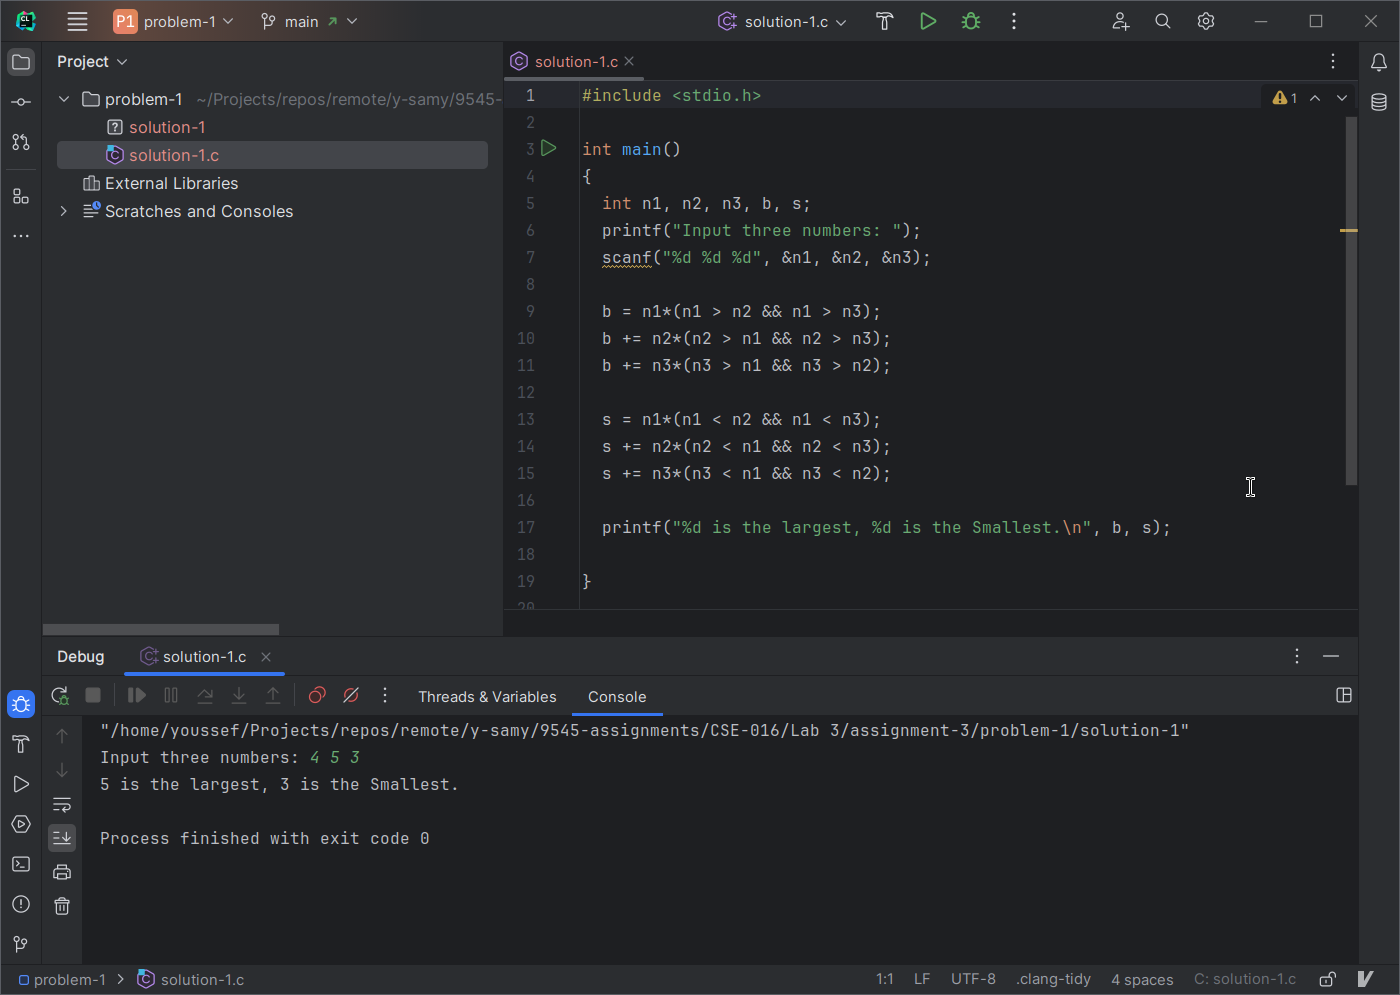
\includegraphics[width=1\linewidth]{prob-1.png}
\ \\\\
\begin{center}
    \textsl{Turn over the page for the last screenshot}
\end{center}
\subsubsection{Problem 2 in CLion}
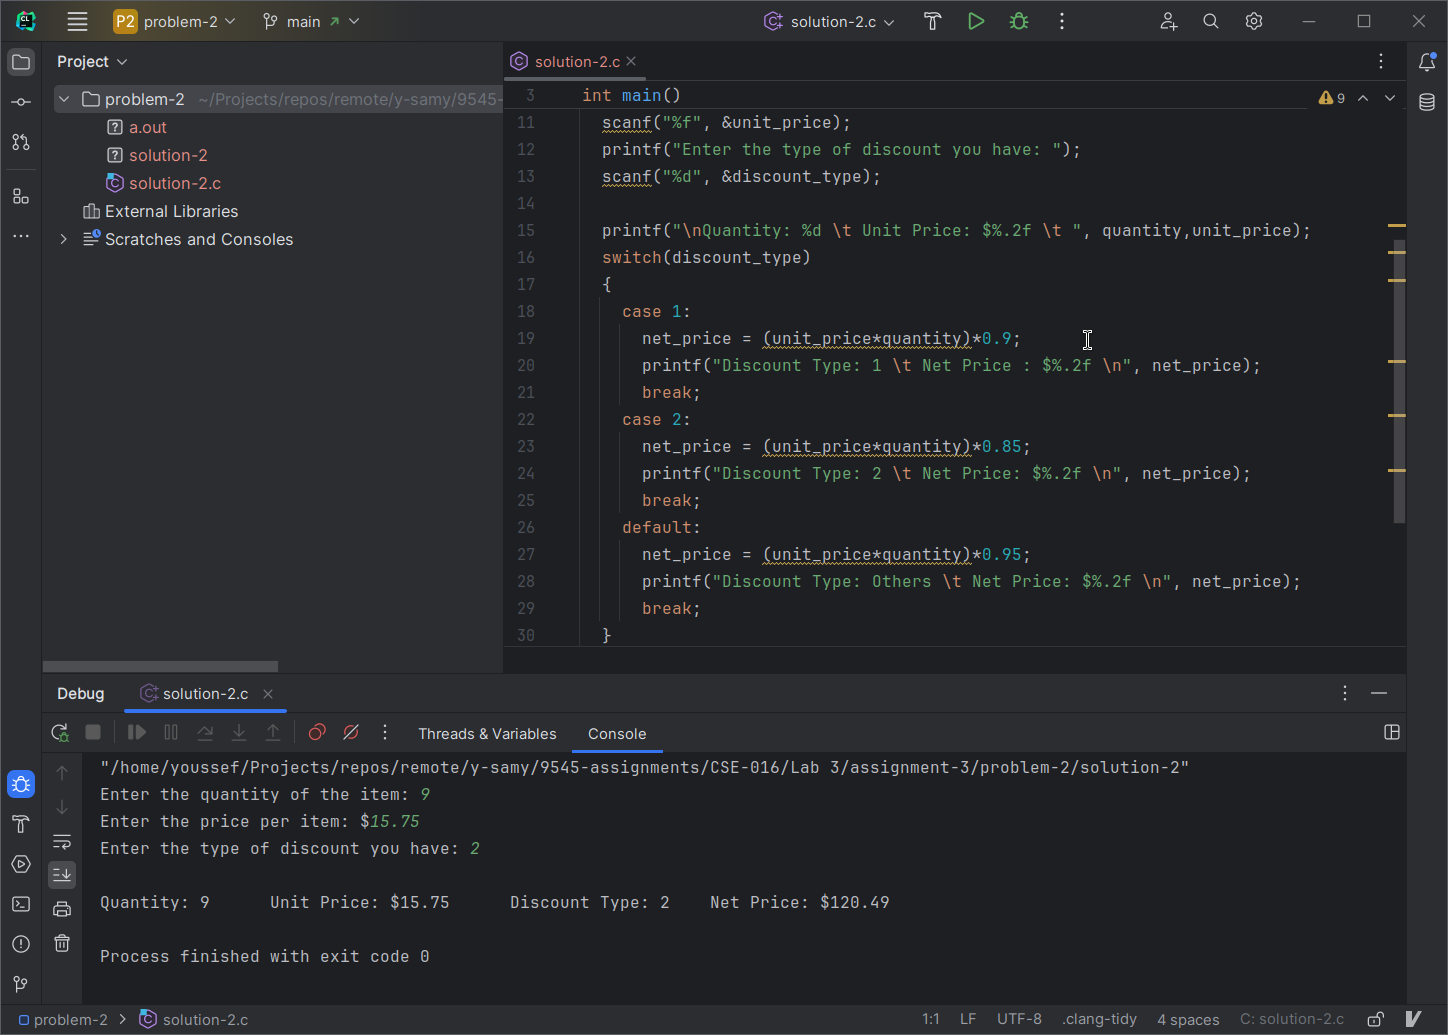
\includegraphics[width=1\linewidth]{prob-2.png}

\subsection{Specifications}
\begin{itemize}
    \item \textbf{Libraries:}
    \begin{itemize}
        \item \texttt{\color{inlinecode}{stdio.h}}
    \end{itemize}
    \item \textbf{Compiler:} GNU C Compiler \texttt{\color{inlinecode}{(gcc)}} version 14.0.1 20240328 (Red Hat 14.0.1-0)
    \item \textbf{C Standard Compatibility}
    \begin{center}
        \begin{tabular}{|c|c|c|c|c|c|}
             \hline
             \textbf{P\#} & \textbf{C89/C90} & \textbf{C99} & \textbf{C11} & \textbf{C17} & \textbf{C23} \\
             \hline
              1 & \checkmark & \checkmark & \checkmark & \checkmark & \checkmark \\
              2 & \checkmark & \checkmark & \checkmark & \checkmark & \checkmark \\
             \hline
        \end{tabular}
    \end{center}
    
    %\begin{flushright}
    %    \begin{tabular}{c|c}
    %         Symbol & Compatibility  \\
    %         \hline
    %         \checkmark & Full \\
    %         $\sim$ & Non-Fatal Errors \\
    %         $\times$ & Incompatible
    %    \end{tabular}
    %\end{flushright}
    \item \textbf{Supported Platforms:} OS: (any), architecture: (any)
    \item \textbf{Tested On:} Fedora 40 Workstation Linux
\end{itemize}
\section{Licenses}
This document, my additions to its \LaTeX \ source code, the software included and its \texttt{C} source code all come without warranty and are all subject to the BSD 3-Clause Open Source License:\\https://opensource.org/license/bsd-3-clause.\\

\begin{center}
    COPYRIGHT \copyright \ 2024, Youssef Ahmed Samy
\end{center}
\fancypagestyle{lastpage}
{
   \fancyhf{}
   \fancyfoot[C]{\textsl{END OF DOCUMENT}}
   \fancyfoot[L]{Assignment 3}
   \fancyfoot[R]{Page \thepage}
}
\thispagestyle{lastpage}
\end{document}
